\secput{poly}{Polygonal Range Queries}


% introduce how to use meta-algorithm to handle irregular range queries,
% including, right triangular queries, arbitrary triangular queries, to
% arbitrary polygonal queries

In this section, we explain how use meta-algorithms
to handle polygonal range query in $2$-D grids efficiently, given all
normals are known at preprocessing time. The examples in this section are
for $2$-D, but we believe that the methodology can be extended to 
higher-dimensions (will be our future work).

\subsecput{triangle}{Triangular Query in $2$-D grid}

\begin{figure*}[t!]
\centering
\subfigure[Preparing for a 1D oblique query that returns partial-sums of trapezoidal regions]{\includegraphics[width=3in]{figures/right-triangles-1.eps}
\label{fig:init-right-triangle-1}}
\hfill
%\hspace{0.01cm}
\subfigure[Decomposing a right triangular query into oblique and rectangular queries]{\includegraphics[width=3in]{figures/right-triangles-2.eps}
\label{fig:init-right-triangle-2}}
\vspace*{-0.5cm}
%\hfill
%\subfigure[Meta-algorithm for right triangular query in $2$-D grid]{\includegraphics[width=2in]{figures/meta_right_triangle.eps}
%\label{fig:meta-right-triangle}}
\caption{Handling right triangular queries with horizontal bases and hypotenuses with a fixed slope.}
\label{fig:right-triangle}
\end{figure*}


We will first consider right triangular queries with fixed slopes.
We assume that the slope of the hypotenuse as well as that of the 
base (or perpendicular) are given during preprocessing time. 

\subsubsecput{rightTri}{Right Triangular Queries with Horizontal Bases}

In this section we show how to decompose a right triangular query with a
horizontal base and a hypotenuse with a fixed slope into three queries:
one 1D \defn{oblique query} (to be explained shortly), one 2D rectangular
query, and one 1D vertical range query.  We already know how to preprocess
the 2D grid to answer the last two queries using a constant number of
semigroup operations. We introduce the notion of oblique queries below,
and explain how to answer them in $O(1)$ semigroup operations, too.

We define oblique queries in a 2D grid $G$ w.r.t. a given straight line
and a given slope $m$.  W.l.o.g. our explanations below assume a vertical
line, say, $L_v$. We consider all lines with slope $m$ that pass thru
at least two grid points, and intersect $L_v$ at a point inside $G$.
Let $L_s$ be such a line (see \figref{init-right-triangle-1}).  If $L_s$
passes thru $k$ grid points (say, $p_0$, $p_1$, \ldots, $p_{k-1}$),
we divide $L_s$ into $k - 1$ segments, where segment $i \in [0, k - 2]$
is the section of the line starting from point $p_i$ and ending right
before point $p_{i+1}$. We will compute a semigroup sum $s_i$ (explained
below) for each segment $i$, and construct a range query data structure
based on these $s_i$ values to allow 1D partial-sum queries on them.
The $s_i$ values are computed as follows. Suppose $L_s$ intersects
$L_v$ at $o$. Consider a horizontal line $L_h$ through $o$. Now $s_i$
is computed based on the location of $p_i$ and $p_{i + 1}$ w.r.t. $L_h$
\punt{$L_v$}:
%
\begin{itemize}
%
\item[-] If $p_i$ is on the right of $L_v$, then $s_i$ is the sum of all
semigroup elements inside the trapezoid containing all grid points on or
below line $p_i p_{i+1}$, on or to the right of the vertical line through
$p_i$, to the left of the vertical line through $p_{i+1}$, and on or above
the horizontal line $L_h$. For example, in \figref{init-right-triangle-1},
$s_3$ is the sum of all grid points on or inside the trapezoid defined
by lines $p_3 p_4$, $p_3 a$, $p_4 c$ and $ac$, except the points on line
$p_4 c$.
%
\item[-] If $p_{i+1}$ is on the left of $L_v$, then $s_i$ is the sum of
all semigroup elements inside the trapezoid containing all grid points on
or to the right of $p_i p_{i+1}$, on or above the horizontal line through
$p_i$, below the horizontal line through $p_{i+1}$, and on or to the left
of $L_v$. For example, in \figref{init-right-triangle-1}, $s_1$ is the
sum of all grid points on or inside the trapezoid defined by lines $p_1
p_2$, $p_1 d$, $p_2 b$ and $bd$, but excluding the points on line $p_2 b$.
%
\item[-] If $p_{i}$ is on the left, but $p_{i+1}$ is on the right
of $L_v$, then $s_i$ is the sum of grid points on or inside the
right triangle defined by points $p_i$, $o$ and line $L_v$, and
the one defined by points $p_{i+1}$, $o$ and line $L_h$, excluding
the points on the vertical line through $p_{i + 1}$. Sum $s_2$ in
\figref{init-right-triangle-1} is an example.
%
\end{itemize}

Now suppose we are given a right triangular query $p_i p_j p$ whose
hypotenuse $p_i p_j$ lies on $L_s$, but $p_i$ and $p_j$ are on the
opposite sides of $L_v$. Then $p_i p_j p$ can be decomposed into
the following three queries (see, e.g., triangle $p_1 p_4 p$ in
\figref{init-right-triangle-2}).
%
\begin{itemize}
%
\item[-] An oblique query on $L_s$ from $p_i$ to $p_j$,
%
\item[-] A 2D query for the rectangular region $ocpd$, where $c$ is
the intersection point of $p_j p$ and $L_h$, and $d$ is the point of
intersection of lines $p_i p$ and $L_v$, and
%
\item[-] A 1D vertical range query from point $p_j$ to point $c$.
%
\end{itemize}
 
Since each of these queries has $O(1)$ complexity, query complexity of
$p_i p_j p$ is also $O(1)$.

An oblique query data structure for the entire grid $G$ can be constructed
as follows. First we vertically or horizontally partition $G$ into two
halves, and contruct a 1D oblique range query data structure for each
line $L_s$ of given slope $m$ that passes thru at least two grid points
and interesects the partition line inside the grid. We then preprocess
the two halves recursively.

In order to answer a right triangular query we first check if the
triangle is completely contained inside one of the two partitions of
$G$. If not, it intersects the partitioning line, and we can answer the
query as explained above. Otherwise, we move into the half that contains
the triangle, and recursively find a partition in which the triangle
intersects the partitioning line, and answer the query accordingly.

We will now analyze the preprocessing time and space required for
constructing the right triangular range query data structure. Our analysis
of preprocessing time will depend on the complexity of computing the
sum of the grid points inside the smallest right triangle of slope $m$
(where $m$ is the slope of the hypotenuse) that can be specified on the
given grid $G$. Observe that the two endpoints of the hypotenuse of such
a triangle will correspond to two consecutive grid points on an oblique
line $L_s$. Let $\Delta$ be the complexity of computing such a sum.

\begin{theorem}
The right triangular range query data structure for a 2D grid of size
$N$ can be constructed in $\Theta( N(\Delta + \log^{2}{N}))$ time and
$\Theta( N \log^{2}{N} )$ space assuming that the hypotenuse of each
query triangle has a fixed slope and the base is horizontal.
\label{thm:rightTri}
\end{theorem}
%
\begin{IEEEproof}(sketch)
%
We first construct a range query data structure for 2D rectangular queries
on the given grid $G$. As we discussed earlier such a data structure can
be constructed in $\Theta( N \log^2{N})$ time and space so that queries
can be answered in $O(1)$ semigroup operations.

Let us now consider the space complexity of the data structure for
oblique queries. We know that an oblique line passing through $k$ grid
points stores $k - 1$ semigroup elements.  Ignoring for the time being
the complexity of computing these elements, we can preprocess such a
line in $\Theta( k \log{k} )$ time and space so that 1D range queries on
those elements can be answered in $O(1)$ time. If we are preprocessing
a 2D grid $G'$ of size $N'$ at a particular level of recursion, then
the preprocessing time and space for all oblique lines for $G'$ in that
level of recursion is $\Theta\left( \sum_{ 0 \leq i < r }{ k_i \log{k_i} }
\right)$, where $r$ is the number of oblique lines and $k_i$ is the number
of grid points on the $i$-th oblique line. Observe that $\sum_{ 0 \leq
i < r }{ k_i } = N'$, and so the complexity above reduces to $\Theta(
N' \log{N'} )$.  Now since $G$ has $N$ points, and it is preprocessed
through $\log{N}$ levels of recursion, the preprocessing time and space
for $G$ is clearly $\Theta( N \log^2{N} )$.

The total time required for computing the semigroup elements (i.e.,
the $s_i$ values, see \figref{init-right-triangle-1}) can be derived as
follows. For each oblique line $L_s$, we first compute the sum of all
grid points inside each smallest triangle with hypotenuse on $L_s$. Since
there are fewer than $N$ such triangles across all oblique lines, the
total time for precomputing all of them is $O( N \Delta )$. Now observe
that the trapezoid below each $s_i$ (see \figref{init-right-triangle-1})
can decomposed into one smallest triangle and a rectangle.  The sum of
the grid points inside the rectangle can be computed in constant time
using the rectangular query data structure we already constructed.
Hence, each $s_i$ can thus be computed in $O(1)$ time.
%
\end{IEEEproof}

Observe that if $B$ and $P$ are the lengths of the base and the
perpendicular, respectively, of a smallest triangle, then $\Delta = O(
min(B, P) )$, as we can use our rectangular query data structure to
perform either $P$ horizontal 1D queries or $B$ vertical queries to
compute the sum inside the triangle. In the worst case, $\Delta = O(
min(B, P) ) = O( \sqrt{N} )$.

\punt{
\begin{figure*}[t!]
\centering
\subfigure[Initial algorithm for right triangular query in $2$-D grid]{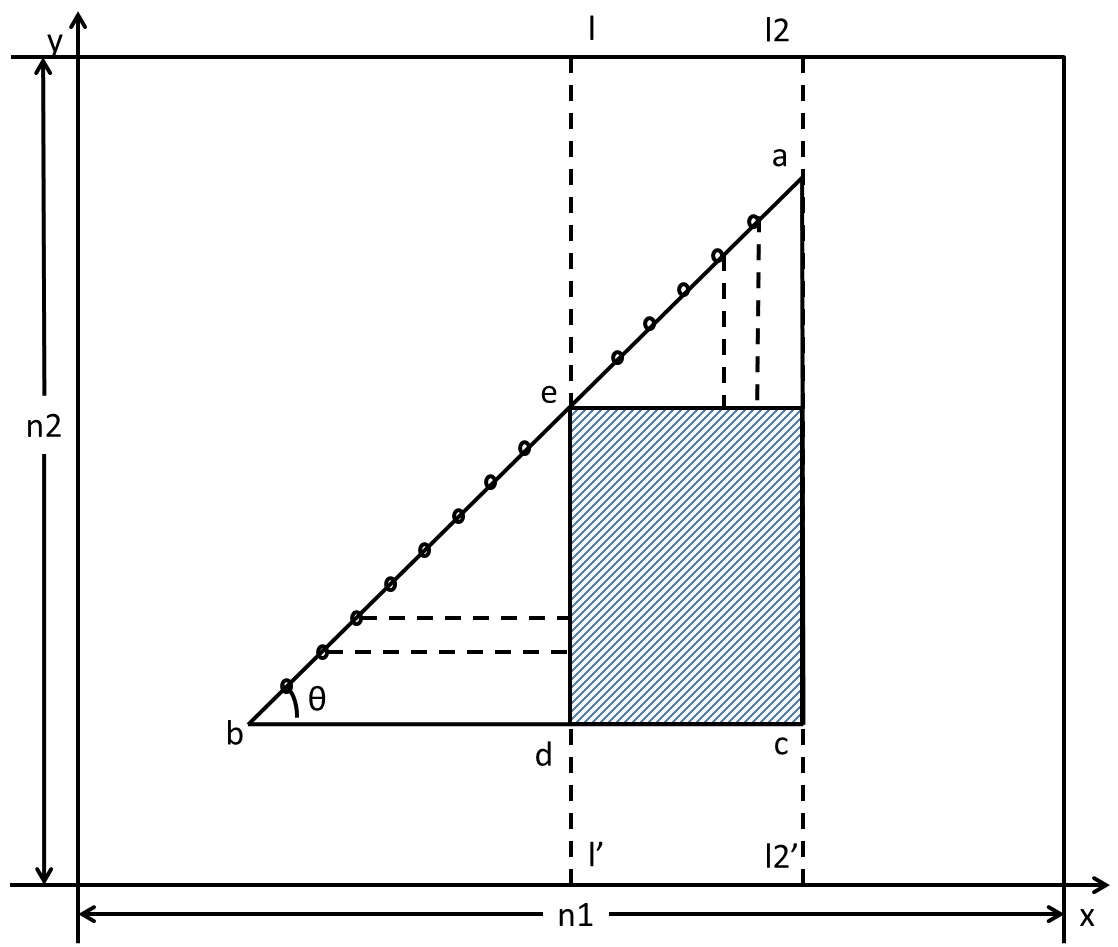
\includegraphics[clip,width=3in]{figures/init_right_triangle.eps}
\label{fig:init-right-triangle}}
\hfill
%\hspace{0.01cm}
\subfigure[Meta-algorithm for right triangular query in $2$-D grid]{\includegraphics[clip,width=3in]{figures/meta_right_triangle.eps}
\label{fig:meta-right-triangle}
}
\caption{Initial and meta-algorithm for right triangular query in $2$-D grid}
\label{fig:right-triangle}
\end{figure*}
} % punt ends

\subsubsection*{Meta algorithm}
% for Right Triangular Query in $2$-D grid}
The meta-algorithm for right triangular query that rectilinear to
axes is very similar to that for rectangular query. So we just use a
triangular preprocessing/query algorithm as the $\id{input\_2D\_algo}$,
then everything remains the same as in meta-algorithm for rectangular
ranges.  \secref{meta-2D} explains more on how meta-algorithm works on 2D
rectangles. \figref{meta-2D} and \figref{meta-right-triangle} provides
a graphical illustration of how the meta-algorithm works on rectangles
and right triangles. More details are omitted from this extended abstract.

\begin{theorem}
If we input the above initial right triangular range preprocessing and
query algorithm to our meta-algorithm and self-apply $\Theta(\alpha^2(N))$,
times, it will achieve $\Theta( N(\Delta + \alpha^{2}{(N)}))$ time and
$\Theta( N \alpha^{2}{(N)} )$ space assuming that the hypotenuse of each
query triangle has a fixed slope and the base is horizontal. The query
overhead will become $\Theta(\alpha^2(N))$.
\label{thm:metaRightTri}
\end{theorem}

\begin{figure*}[t!]
\centering
\subfigure[A right triangle with an oblique base]{
\includegraphics[width=2in]{figures/rotated-right-triangles-1.eps}
\label{fig:init-rotated-right-triangle-1}}
\hfill
%\hspace{0.01cm}
\subfigure[Rotating the input grid to make the triangle base horizontal, and embedding it in a finer grid with axis-parallel sides]{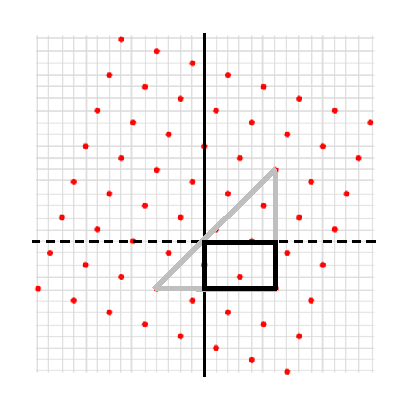
\includegraphics[width=2in]{figures/rotated-right-triangles-2.eps}
\label{fig:init-rotated-right-triangle-2}}
\hfill
\subfigure[Oblique queries in the fine grid]{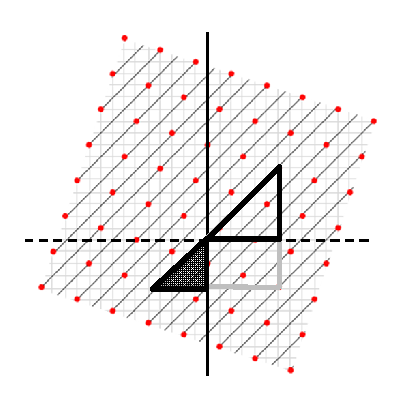
\includegraphics[width=2in]{figures/rotated-right-triangles-3.eps}
\label{fig:init-rotated-right-triangle-3}}
\caption{Handling right triangular queries with a fixed hypotenuse slope but without horizontal bases.}
\label{fig:rotated-right-triangle}
\end{figure*}


\subsubsecput{rightTriOblique}{Right Triangular Queries without Horizontal Bases}
%
In this section we consider right triangular queries that have fixed
slopes for all sides, but the base is neither horizontal nor vertical.
We define the \defn{feature size} of a straight line passing thru a
grid as the distance between two consecutive grid points lying on that
line. Let $\delta_b$, $\delta_p$ and $\delta_h$ be the feature sizes
of base, perpendicular and hypotenuse, respectively, of any query
triangle. For example, in \figref{init-rotated-right-triangle-1},
$\delta_b = \delta_p = \sqrt{10}$ and $\delta_h = \sqrt{5}$. We assume
that $\delta_b$ and $\delta_p$ are small constants.

Assuming that the original grid has $N$ points, we can rotate the grid
so that query base becomes horizontal, and embed it in an axis-parallel
finer grid of size $\Theta( N \delta_b \delta_p )$ so that every
point of the original grid sits on a grid point of the finer grid
(see \figref{init-rotated-right-triangle-2}).  Since $\delta_b$ and
$\delta_p$ are assumed to be constants, we can use our algorithm from
\secref{rightTri} to solve right triangular range queries on this grid
within the performance bounds proved in \thmref{rightTri}.

\begin{figure*}[t!]
\centering
\subfigure[An arbitrary triangle in a 2D grid]{
\includegraphics[width=2in]{figures/arbitrary-triangles-1.eps}
\label{fig:init-arbitrary-triangle-1}}
\hfill
%\hspace{0.01cm}
\subfigure[Rotating the grid to make the largest side of the triangle horizontal, and embedding the input grid in a finer grid with axis-parallel sides]{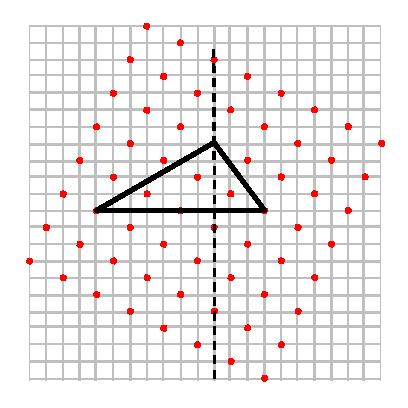
\includegraphics[width=2in]{figures/arbitrary-triangles-2.eps}
\label{fig:init-arbitrary-triangle-2}}
\hfill
%\hspace{0.01cm}
\subfigure[Decomposing an arbitrary polygonal query into rectangles and triangles using only horizontal and vertical lines]{
\includegraphics[width=2in]{figures/polygonal.eps}
\label{fig:init-polygonal}}
\caption{Handling arbitrary triangular and polygonal queries with fixed slopes.}
\label{fig:rotated-arbitrary-triangle}
\end{figure*}

\subsubsecput{arbitraryTri}{Arbitrary Triangular Query in a $2$-D grid}
%
We consider arbitrary triangular queries on a 2D grid (see
\figref{init-arbitrary-triangle-1}) with fixed slopes for all sides.
We take the largest side $b$ of such a triangle, and rotate the grid so
that $b$ becomes horizontal. We embed the rotated grid in a finer grid
as in \secref{rightTriOblique} (see \figref{init-arbitrary-triangle-1}).
Let us draw a perpendicular $p$ on $b$ from the triangle vertex that
does not lie on $b$. Now assuming that the feature sizes of $b$ and
$p$ are small constants the size of the finer grid will be within a
constant factor of the size of the original grid. The perpendicular $p$
divides the query triangle into two right triangles, and thus the given
triangular query can decomposed into two right triangular queries, and
we can preprocess the finer grid to answer them within the performance
bounds proved in \thmref{rightTri}.

\subsecput{polygon}{Polygonal Query in a $2$-D grid}
%
We now consider arbitrary query polygons with sides that can have slopes
from a fixed set of slopes known during preprocessing time. We assume that
lines corresponding to these slopes have small constant feature sizes.
The key issue is decomposing this polygon into rectangles and triangles
without introducing any additional slopes. First we draw horizontal lines
through each vertex of the polygon which decompose the polygon into a set
of disjoin triangles and trapezoids (see \figref{init-polygonal}). Then we
use vertical lines to decompose each trapezoid into at most one rectangle
and no more than two right triangles. The total number of triangles and
rectangles thus created is within a constant factor of the total number
vertices in the original polygon. We now create a query data structure
for each triangle and rectangles. If the polygon has only a constant
number of vertices the performance bounds given in \thmref{rightTri} hold.

\punt{
\subsecput{extensionToHigherD}{Extension to Higher Dimensions}
%
It is not difficult to extend our 2D algorithm for right triangular
queries to trirectangular tetrahedronal queries in 3D. In a
trirectangular tetrahedron the three face angles at one vertex 
are right angles. The face opposite the vertex of the right angles 
is called the base. Similar to oblique lines parallel to
the hypotenuse of a right triangle (see \figref{right-triangle}),
we create oblique planes parallel to the base of the
trirectangular tetrahedron.  
}
% punt ends
